\section{Analiza konkurencyjnych rozwiązań}

\phantom{Th}

Na rynku znajduje się wiele narzędzi do organizacji czasu, ale \textbf{kalendarz Google} pozostaje niekwestionowanym liderem.
Jest to profesjonalne i przede wszystkim darmowe, preinstalowane narzędzie na większości urządzeń z systemem Android.
Według raportu stworzonego przez zespół pracujący dla DataReportal, w Polsce na rok 2023, aż 87\% użytkowników posiada
telefon właśnie z tym systemem
\cite{datareportal}. Aplikacja ta stanowi nieodłączny element funkcjonowania firm, zwłaszcza tych początkujących,
ale nie tylko. Ułatwia harmonogramowanie spotkań, śledzenie projektów i pozwala na zachowanie kontroli nad terminami.
Dużym atutem kalendarza Google jest rozdzielenie zadań i wydarzeń na osobne elementy kalendarza (Rys. \ref{fig:googleCalendar}).\\

\begin{figure}[ht]
  \begin{minipage}{0.4\textwidth}
    \centering
    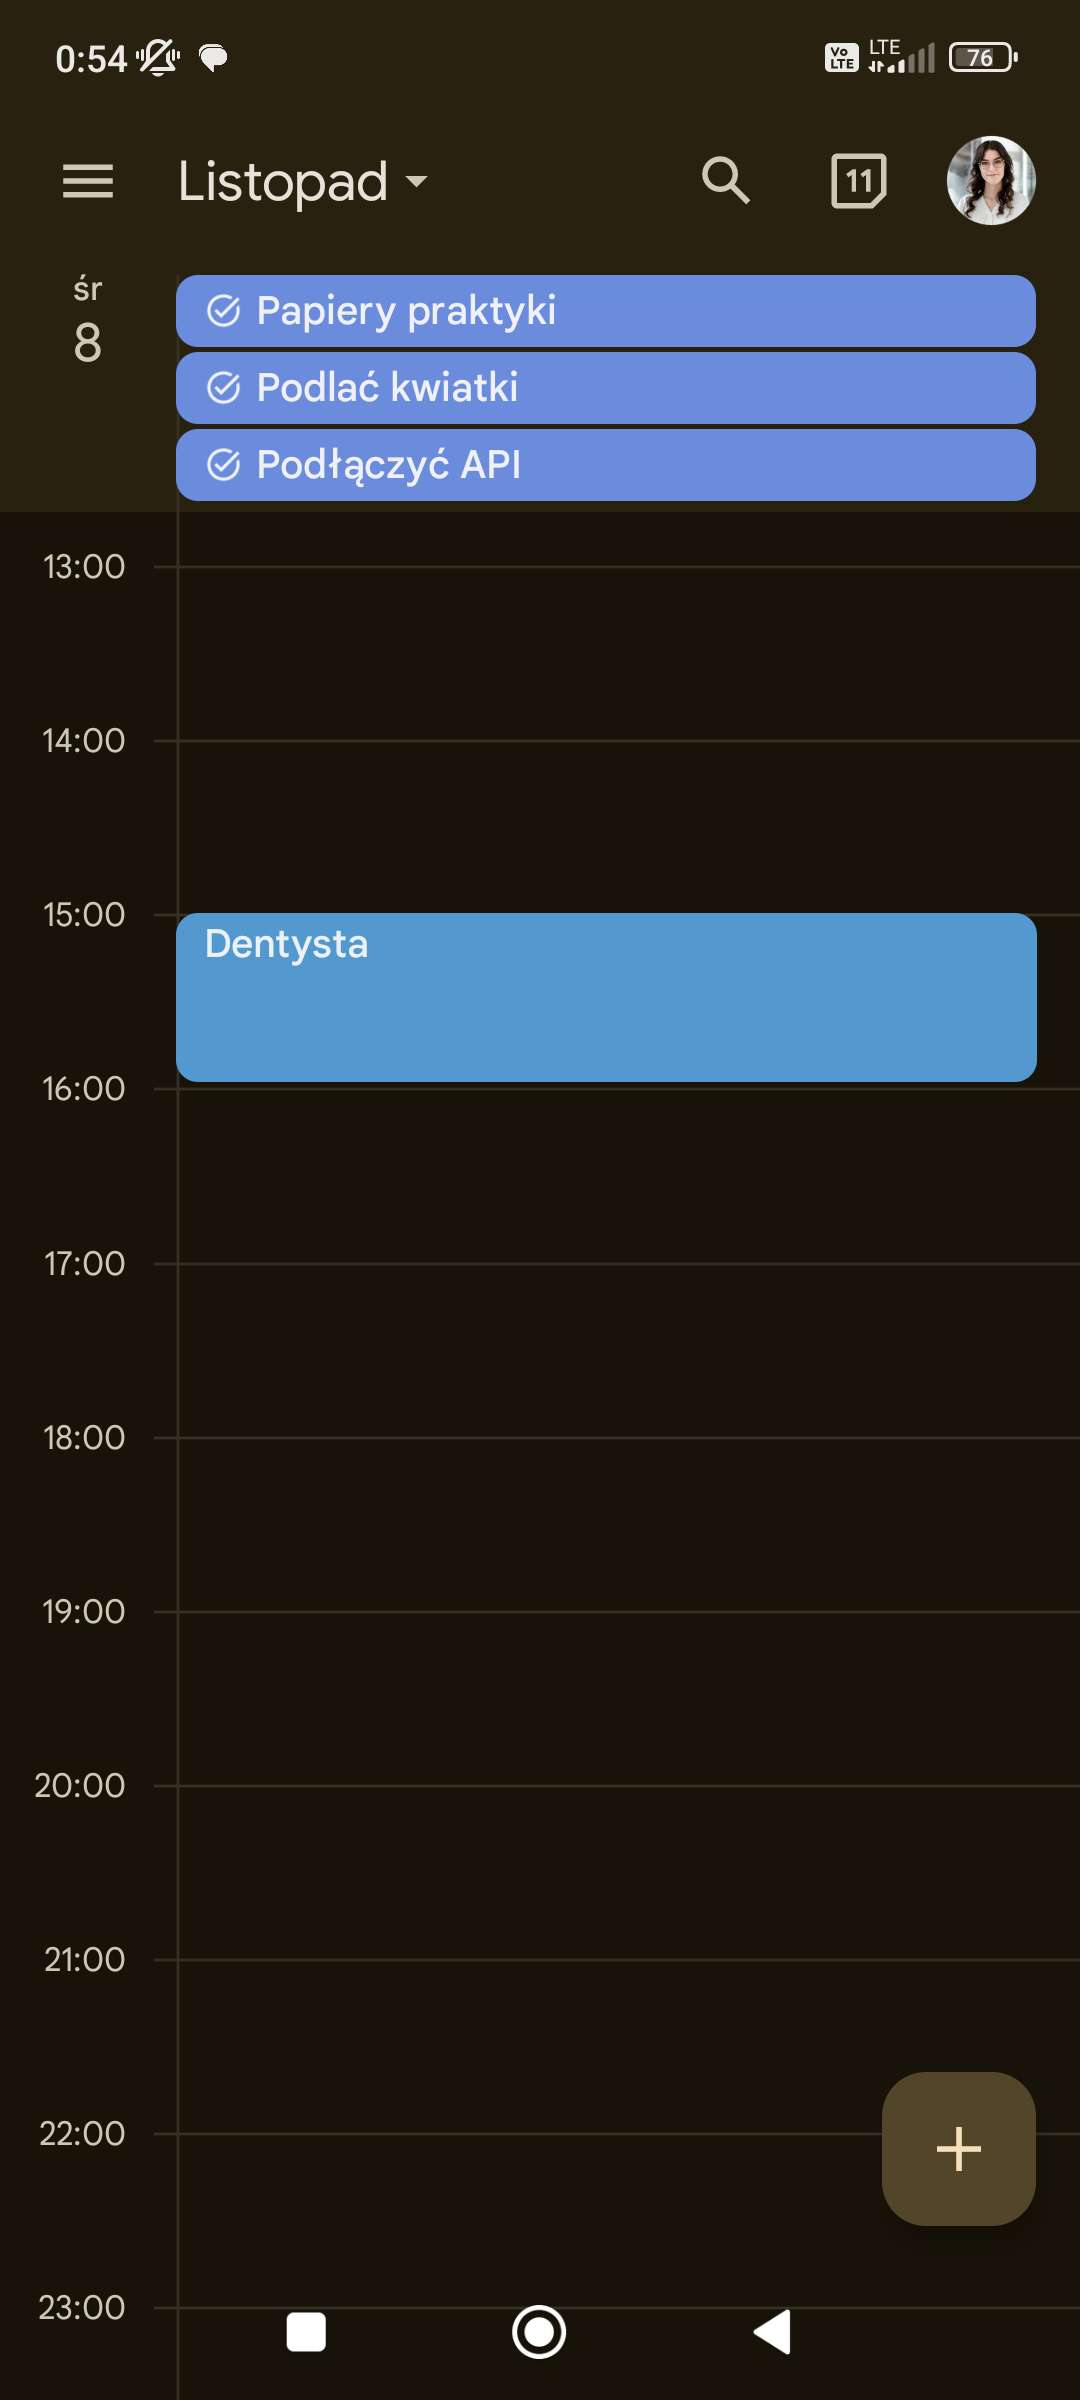
\includegraphics[height=13cm, keepaspectratio]{images/analiza/googleCalendar}
    \caption{Widok konkretnego dnia w kalendarzu Google}
    \label{fig:googleCalendar}
  \end{minipage}
  \hfill
  \begin{minipage}{0.4\textwidth}
    \centering
    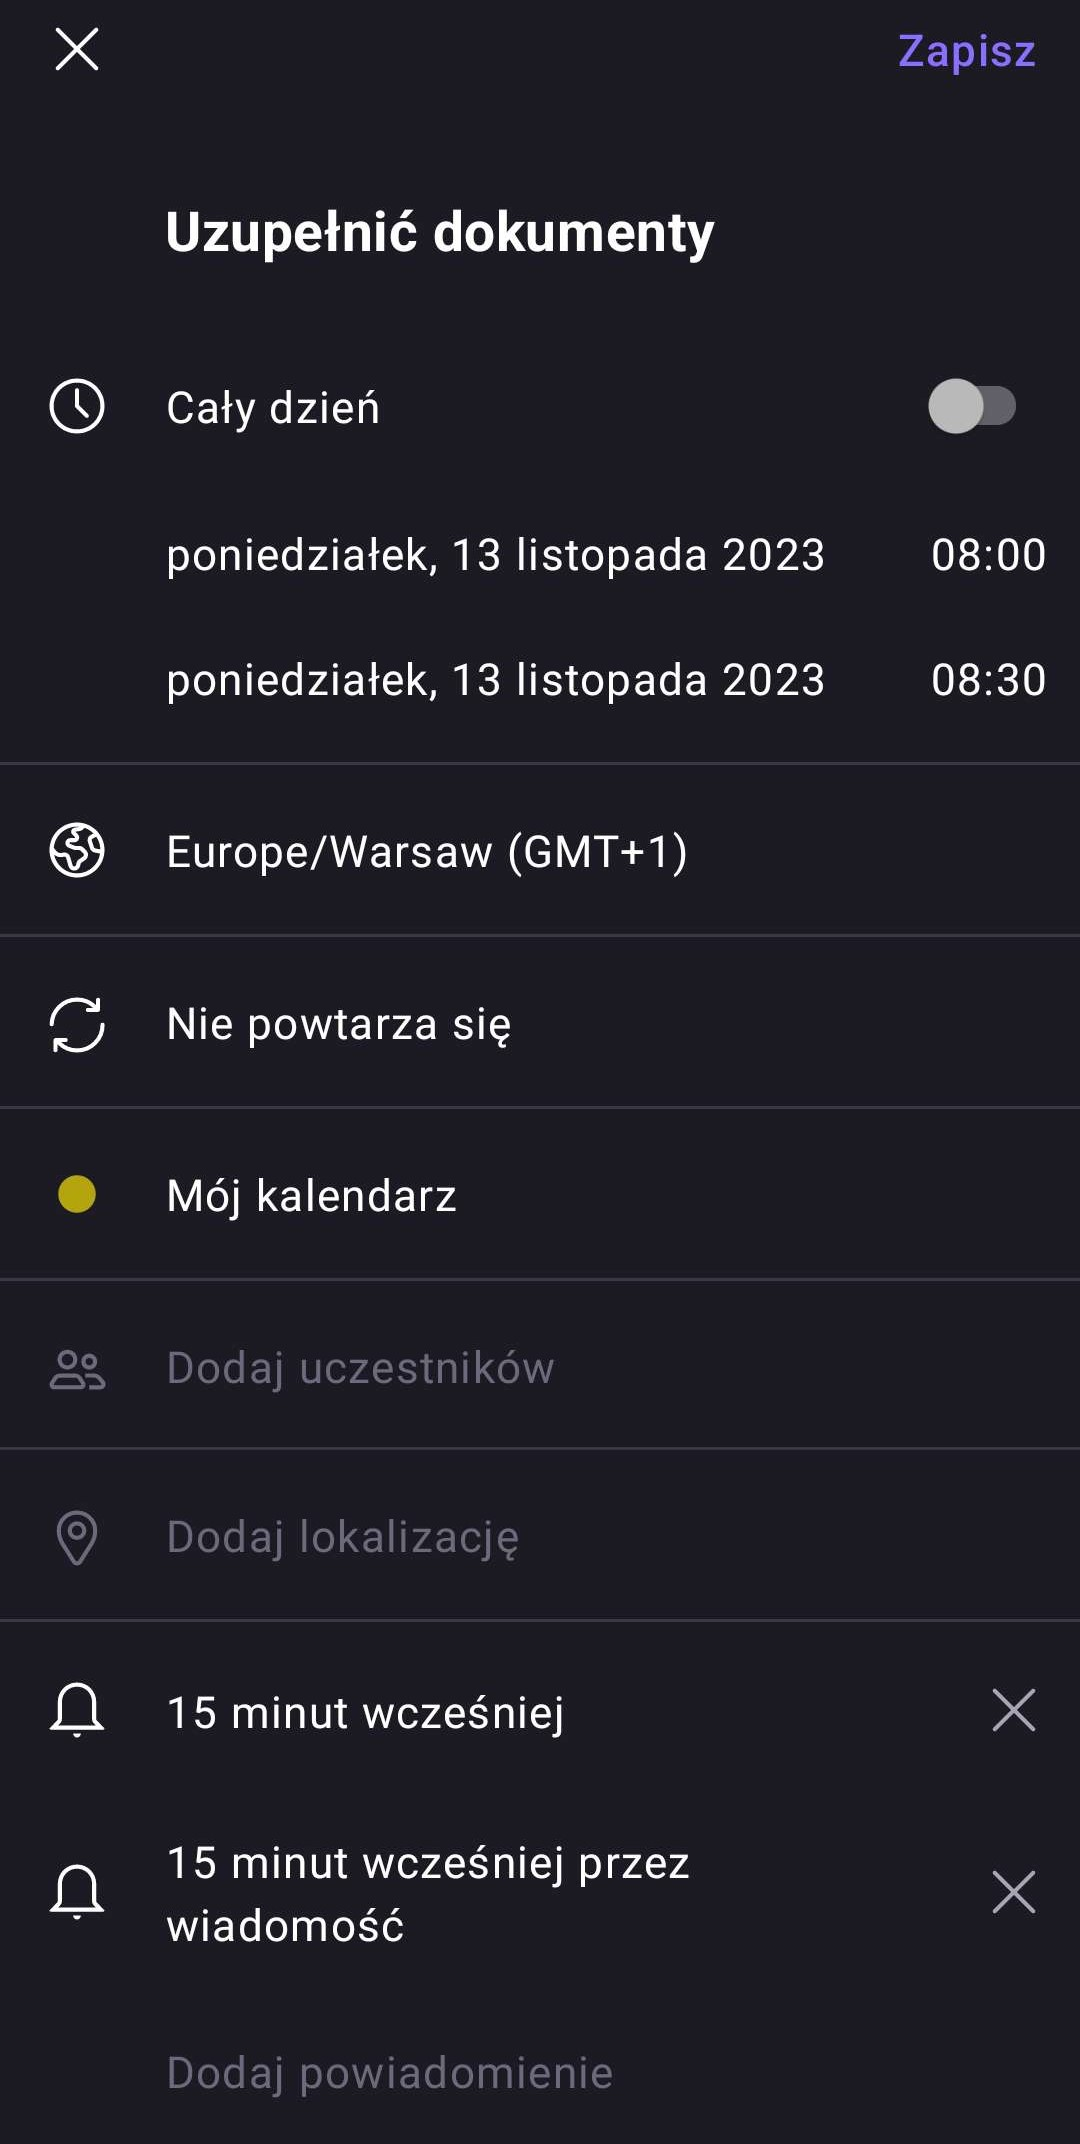
\includegraphics[height=13cm, keepaspectratio]{images/analiza/protonCalendar}
    \caption{Widok tworzenia wydarzenia w kalendarzu Proton}
    \label{fig:protonCalendar}
  \end{minipage}
\end{figure}

Jest to narzędzie umożliwiające precyzyjne określenie wszelkich informacji odnośnie danego wydarzenia.
Nie da się kwestionować, że możliwości jakie daje nam aplikacja są niepotrzebne,
jednakże z punktu widzenia użytkownika końcowego ZodiaCal funkcje takie jak lokalizacja wydarzenia,
link do rozmowy wideo, czy określanie trwania każdego jednego wpisanego wydarzenia od do jest zbędne.
W ZodiaCal istotne jest sprawne dodawanie wydarzeń do kalendarza, bez konieczności przeglądania dodatkowych opcji.\\

Dobrą alternatywą dla kalendarza Google jest \textbf{Proton Calendar} (Rys. \ref{fig:protonCalendar}).
Jest to również zaawansowana aplikacja do monitorowania wydarzeń, z tą różnicą,
iż proton specjalizuje się w zapewnianiu jeszcze większej prywatności i bezpieczeństwa użytkowników.
Z tym, że nie rozróżnia wydarzeń od zadań. Proton to firma oferująca usługi związane
z prywatnością online, w tym bezpiecznymi skrzynkami e-mail i kalendarzami.\\


Bardzo ciekawym i minimalistycznym rozwiązaniem jest aplikacja \textbf{135 To Do List} która poprzez swój estetyczny
i prosty interfejs ułatwia użytkownikom priorytetyzacja zadań na konkretny dzień.
Posiada możliwość zmiany kolejności wpisanych już wcześniej zadań oraz widok całego miesiąca.
Niestety nie ma opcji dodawania cyklicznych wydarzeń. ZodiaCal przyświeca niemalże ta sama minimalistyczna
idea tworzenia interfejsu, jednak wprowadza rozbudowane funkcje, takie jak codzienny horoskop i osobisty dziennik pielęgnacji (Rys. \ref{fig:ToDoList}).\\

\textbf{FeelingMySkin} to bardzo rozbudowane narzędzie do precyzyjnego określenia pielęgnacji cery i nie tylko.
Korzystając z niej użytkownik może układać plany pielęgnacyjne z wykorzystaniem konkretnych produktów,
których używa na co dzień,  monitorować zmiany skórne, czy chociażby śledzić daty przydatności produktów.
To z pewnością przydatna aplikacja, jednakże wymaga czasu, aby opanować wszystkie możliwe funkcje.
Interfejs strony głównej jest bardzo przeładowany informacjami, co utrudnia korzystanie z aplikacji w sposób efektywny (Rys. \ref{fig:feelingMySkin}).\\

\begin{figure}[ht]
  \begin{minipage}{0.4\textwidth}
    \centering
    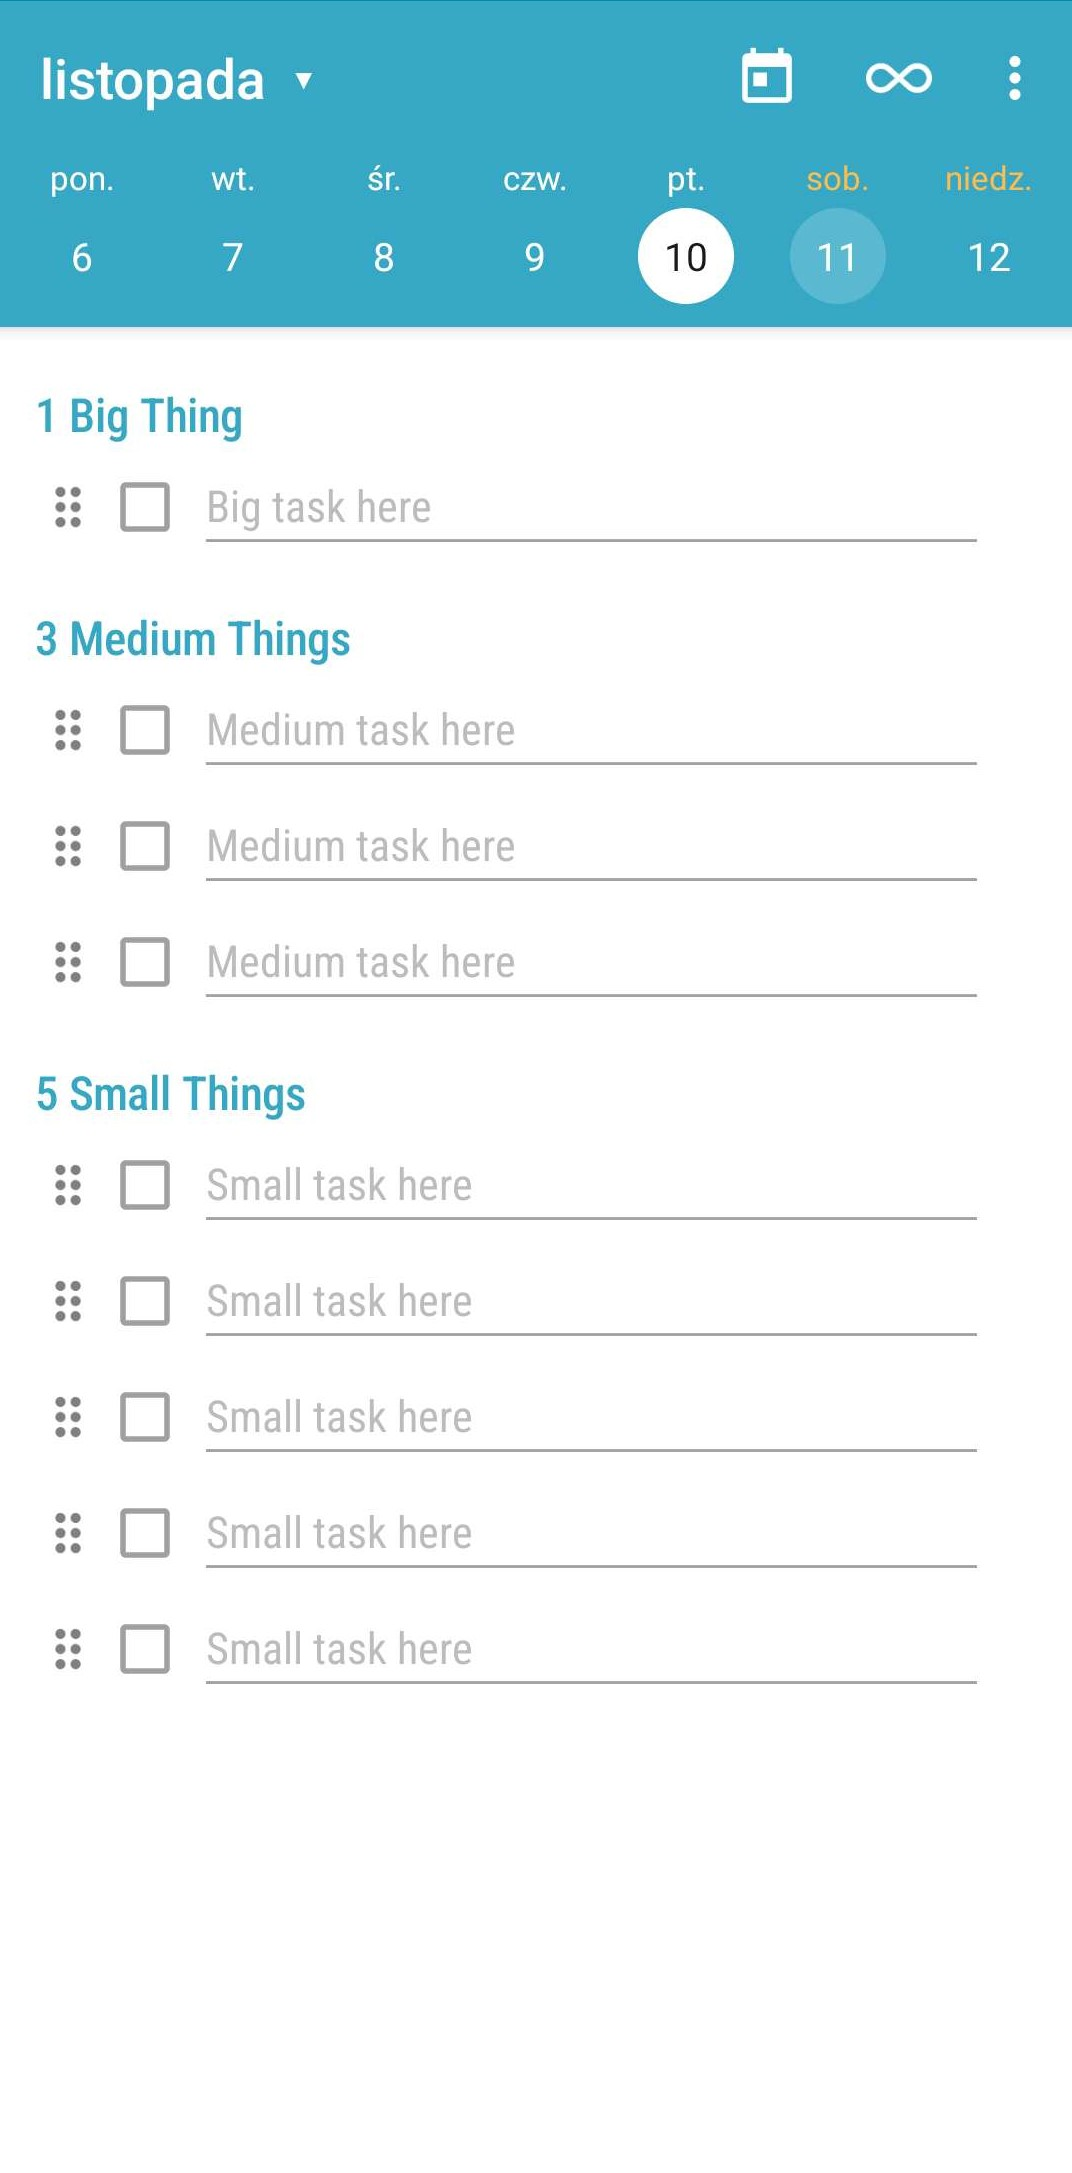
\includegraphics[height=13cm, keepaspectratio]{images/analiza/135ToDoList}
    \caption{Ekran główny aplikacji 135 To Do List}
    \label{fig:ToDoList}
  \end{minipage}
  \hfill
  \begin{minipage}{0.4\textwidth}
    \centering
    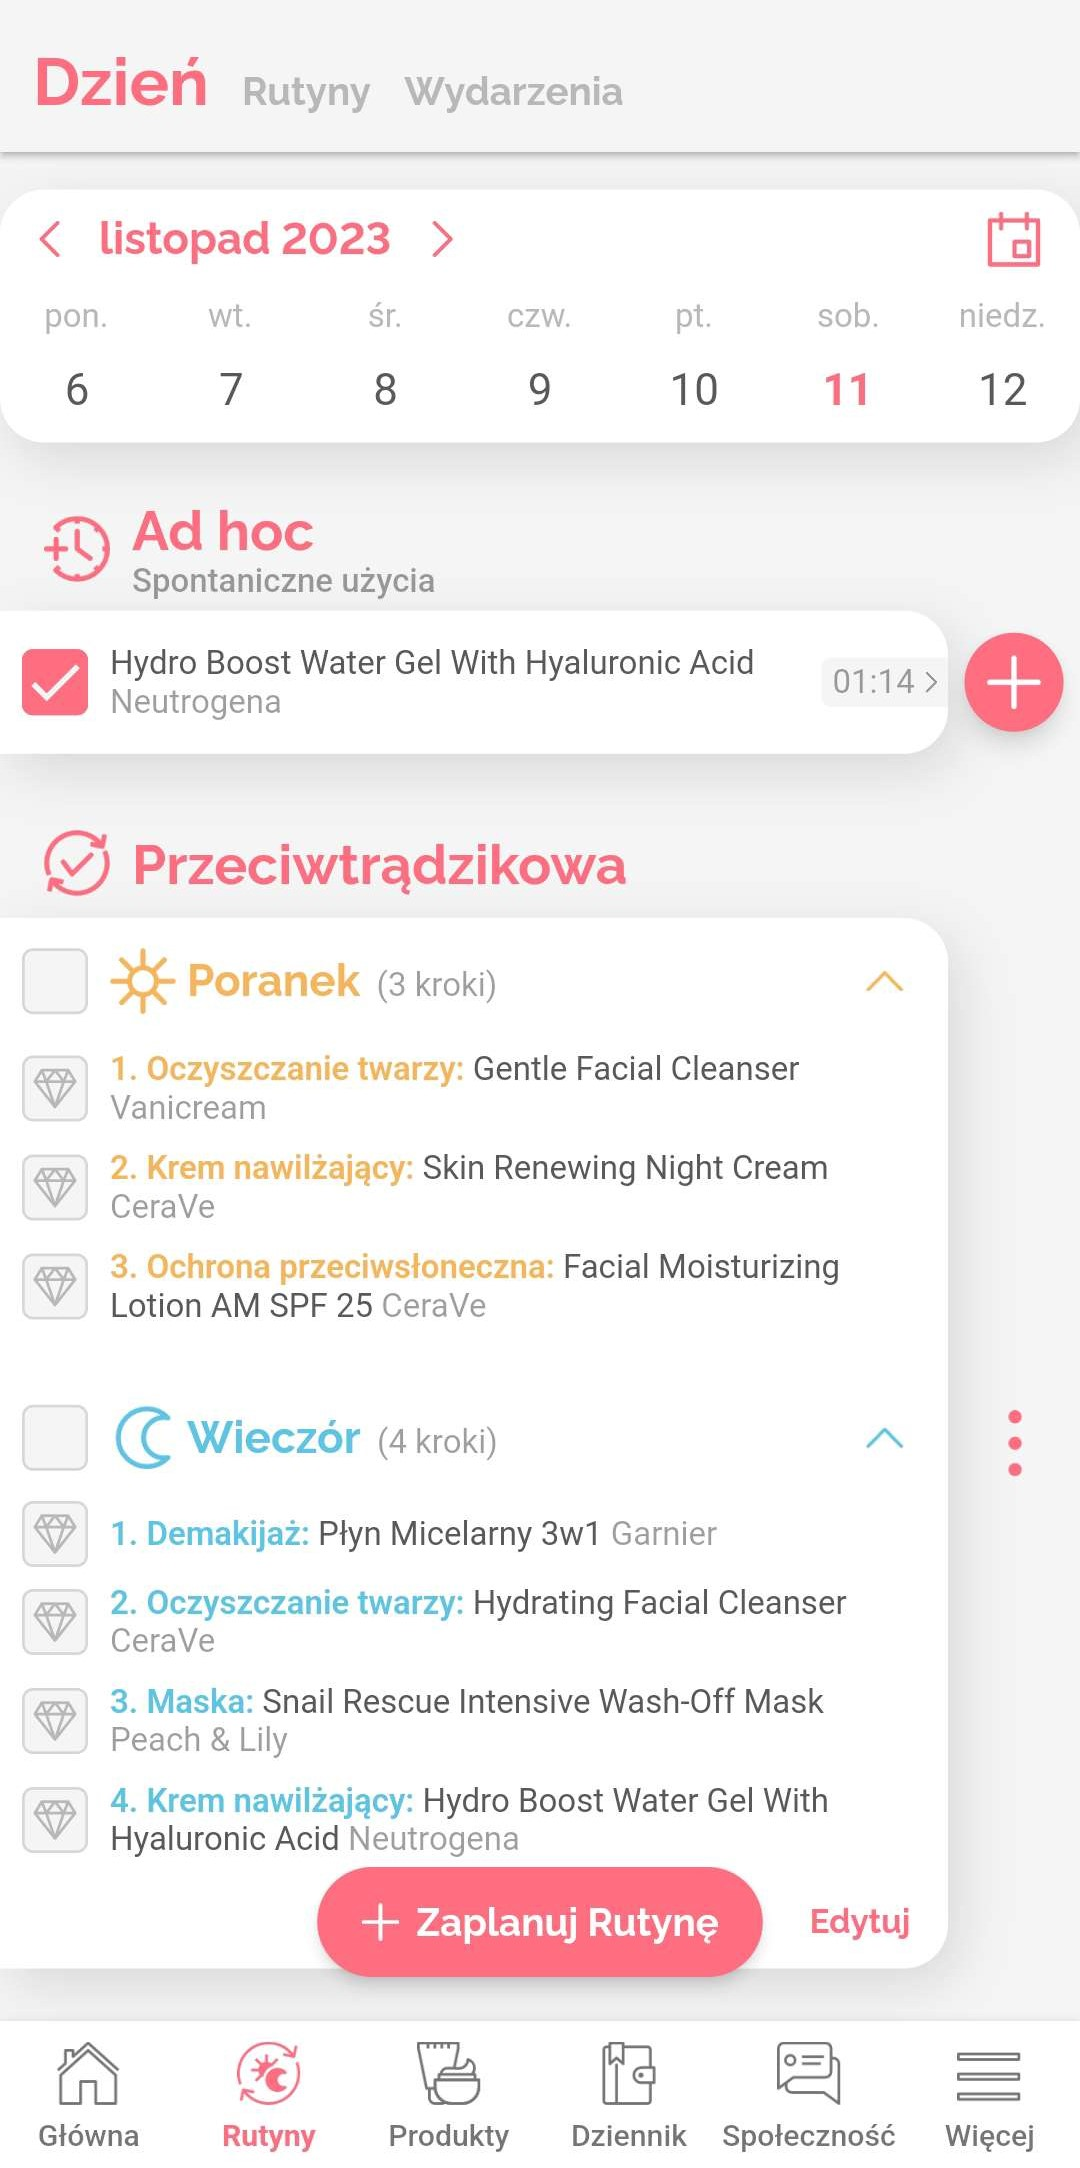
\includegraphics[height=13cm, keepaspectratio]{images/analiza/feelingMySkin}
    \caption{Widok codziennej rutyny w aplikacji FeelingMySkin}
    \label{fig:feelingMySkin}
  \end{minipage}
\end{figure}

ZodiaCal to hybryda wszystkich wymienionych aplikacji.
To minimalistyczne narzędzie służące do wielu celów, ale w podstawowym zakresie.
Próbuje połączyć najlepsze cechy różnych istniejących aplikacji,
oferując minimalistyczny interfejs do zarządzania czasem, zadaniami i nie tylko.
Chociaż nie zawiera wszystkich zaawansowanych funkcji dostępnych w innych aplikacjach,
dąży do dostarczenia użytkownikom wyważonego narzędzia do pracy.


\section{Analiza SWOT}
Napisać tutaj coś o analizie SWOT

\phantom{Th}

\textbf{Mocne strony (Strengths):}\\
•	Prostota: Aplikacja łączy w sobie wyłącznie najpotrzebniejsze funkcje typowego, biurowego kalendarza i dzienniczka pielęgnacji, przez co jest bardziej przystępna dla początkujących.\\
•	Spersonalizowana pielęgnacja: Możliwość dostosowywania rutyn pielęgnacyjnych do konkretnych potrzeb użytkownika.\\
•	Powiadomienia i przypomnienia: Ułatwia utrzymanie regularności w dbaniu o cerę.\\
•	Uczenie maszynowe: Propozycje pielęgnacji na podstawie wcześniejszych danych.\\
•	Wieloplatformowość: Aplikacja działa na wielu platformach dzięki czemu można dotrzeć do szerszej grupy użytkowników.\\

\textbf{Słabe strony (Weaknesses):}\\
•	Brak bazy danych produktów: W aplikacji nie ma możliwości zaciągnięcia z bazy danych kosmetyków, których użytkownik używa podczas pielęgnacji.\\
•	Brak synchronizacji z pocztą: Jeśli użytkowni otrzyma maila odnośnie jakiegoś wydarzenia, nie doda się ono automatycznie do kalendarza.\\

\textbf{Szanse (Opportunities):}\\
•	Rynek pielęgnacji cery: W ostatnich czasach zainteresowanie świadomą pielęgnacją skóry wzrosło co stwarza możliwość przyciągnięcia nowych użytkowników.\\
•	Wprowadzenie płatnej wersji z dodatkowymi funkcjami: Możliwość wprowadzenia płatnej wersji aplikacji z rozszerzonymi funkcjami dla zaawansowanych użytkowników.\\

\textbf{Zagrożenia (Threats):}\\
•	Prywatność i bezpieczeństwo danych: Konieczność zapewnienia wysokiego poziomu ochrony danych użytkowników, zwłaszcza w obszarze związanym z informacjami o pielęgnacji skóry.\\
•	Zmiany w regulacjach dotyczących prywatności: Zmiany przepisów dotyczących ochrony danych osobowych mogą wpłynąć na wymogi dotyczące zachowania prywatności użytkowników i mogą wymagać dostosowania polityki prywatności aplikacji.\\

\section{Analiza przedmiotowa MoSCoW}

MUST
•	Funkcja logowania i rejestracji – połączenie z bazą danych
•	Funkcjonalności związane z kalendarzem 
o	CRUD wydarzeń 
o	Widok roczny
o	Widok miesięczny
o	Widok tygodniowy 
•	Automatyczne uzupełnianie pól cyklicznych wydarzeń w kalendarzu praca/studia
•	Funkcja przydzielania znaku zodiaku z podanej daty przez użytkownika podczas rejestracji 
•	Dzienny horoskop – połączenie z API (RTK-query)
SHOULD
•	Funkcjonalność związana z dodawaniem produktów do danej pielęgnacji 
•	Funkcjonalność związana z zarejestrowaniem danej pielęgnacji na dzień
•	Formularz zgłaszania błędów w aplikacji 
•	Logowanie kontem Google
COULD
•	Analiza pielęgnacji – wykresy 
•	Onboarding zaraz po zarejestrowaniu konta 
•	Powiadomienia 
•	Traker samopoczucia, snu i nawyków
•	Możliwość zmiany języka


WON’T
•	Personalizacja motywów (kolory interfejsu)
•	Wersja na zegarek – możliwość nadzoru pielęgnacji 
•	Propozycja pielęgnacji po 3 miesiącach korzystania aplikacji 
